% textidote: ignore begin
\subsection{Architecture}\label{subsec:architecture}
% textidote: ignore end

The diagram in Figure~\ref{fig:architecture-overview} shows a top-level overview of the system architecture.
It shows how the system is divided into two different development environments, a front end and a back end.
The front end is using~\url{Next.js}, which is a framework for React.
The back end is using Java with Spring Boot.
It is also connected to a PostgreSQL database.

The diagram in Figure~\ref{fig:architecture-backend} shows the back-end architecture.
It is a lot more detailed than the top-level overview.
The back end is split in a business layer and a data access layer.
The business layer is where the controllers are located.
The controllers are responsible for handling the requests from the front end using the REST API.\@
One special controller is the ``CSV File POST'' controller, which is responsible for handling the CSV files that
are uploaded to the system from the front end.
This is necessary to handle the sales data from the~\acrshort{epos} system.
That controller is connected to a batch processor in the data access layer.
The batch processor is responsible for processing the CSV files from comma separated values to database entries.
By using a batch processor, the system can handle large amounts of data without compromising performance.
The other controllers are connected to repositories in the data access layer.
These repositories are responsible for handling the database queries.
Lastly, the data access layer also contains models for the database entries and a logger for logging errors.
Both the batch processor and the repositories are connected directly to the database.
The batch processor is inputting data into the database, while the repositories are querying the database for data.
This keeps the database secure and reliable.

\begin{figure}[h]
    \centering
    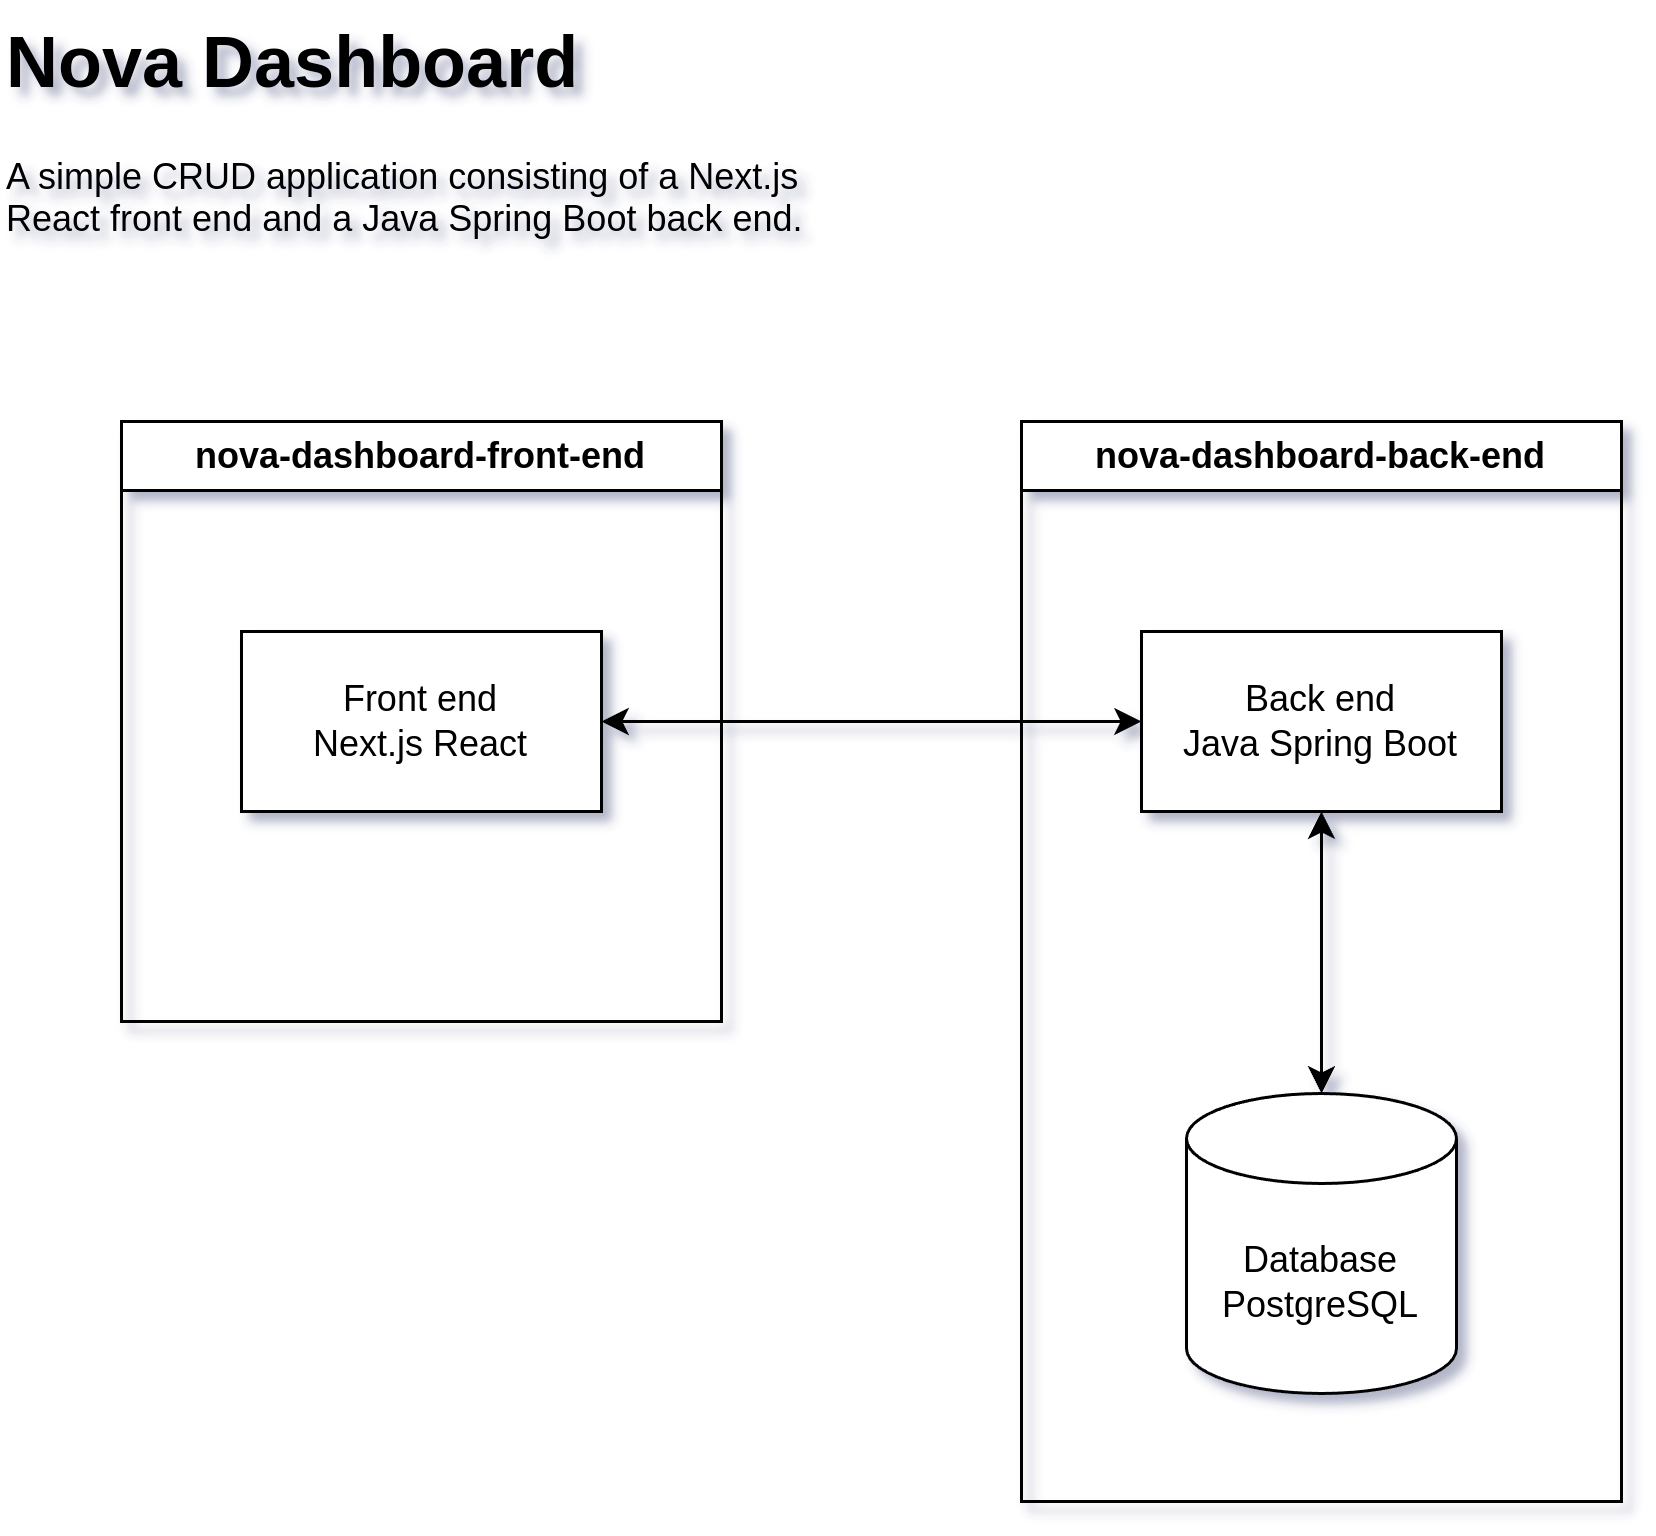
\includegraphics[width=.5\textwidth]{architecture-overview.png}
    \caption{An overview of the system architecture.
    }\label{fig:architecture-overview}
\end{figure}

\begin{figure}[h]
    \centering
    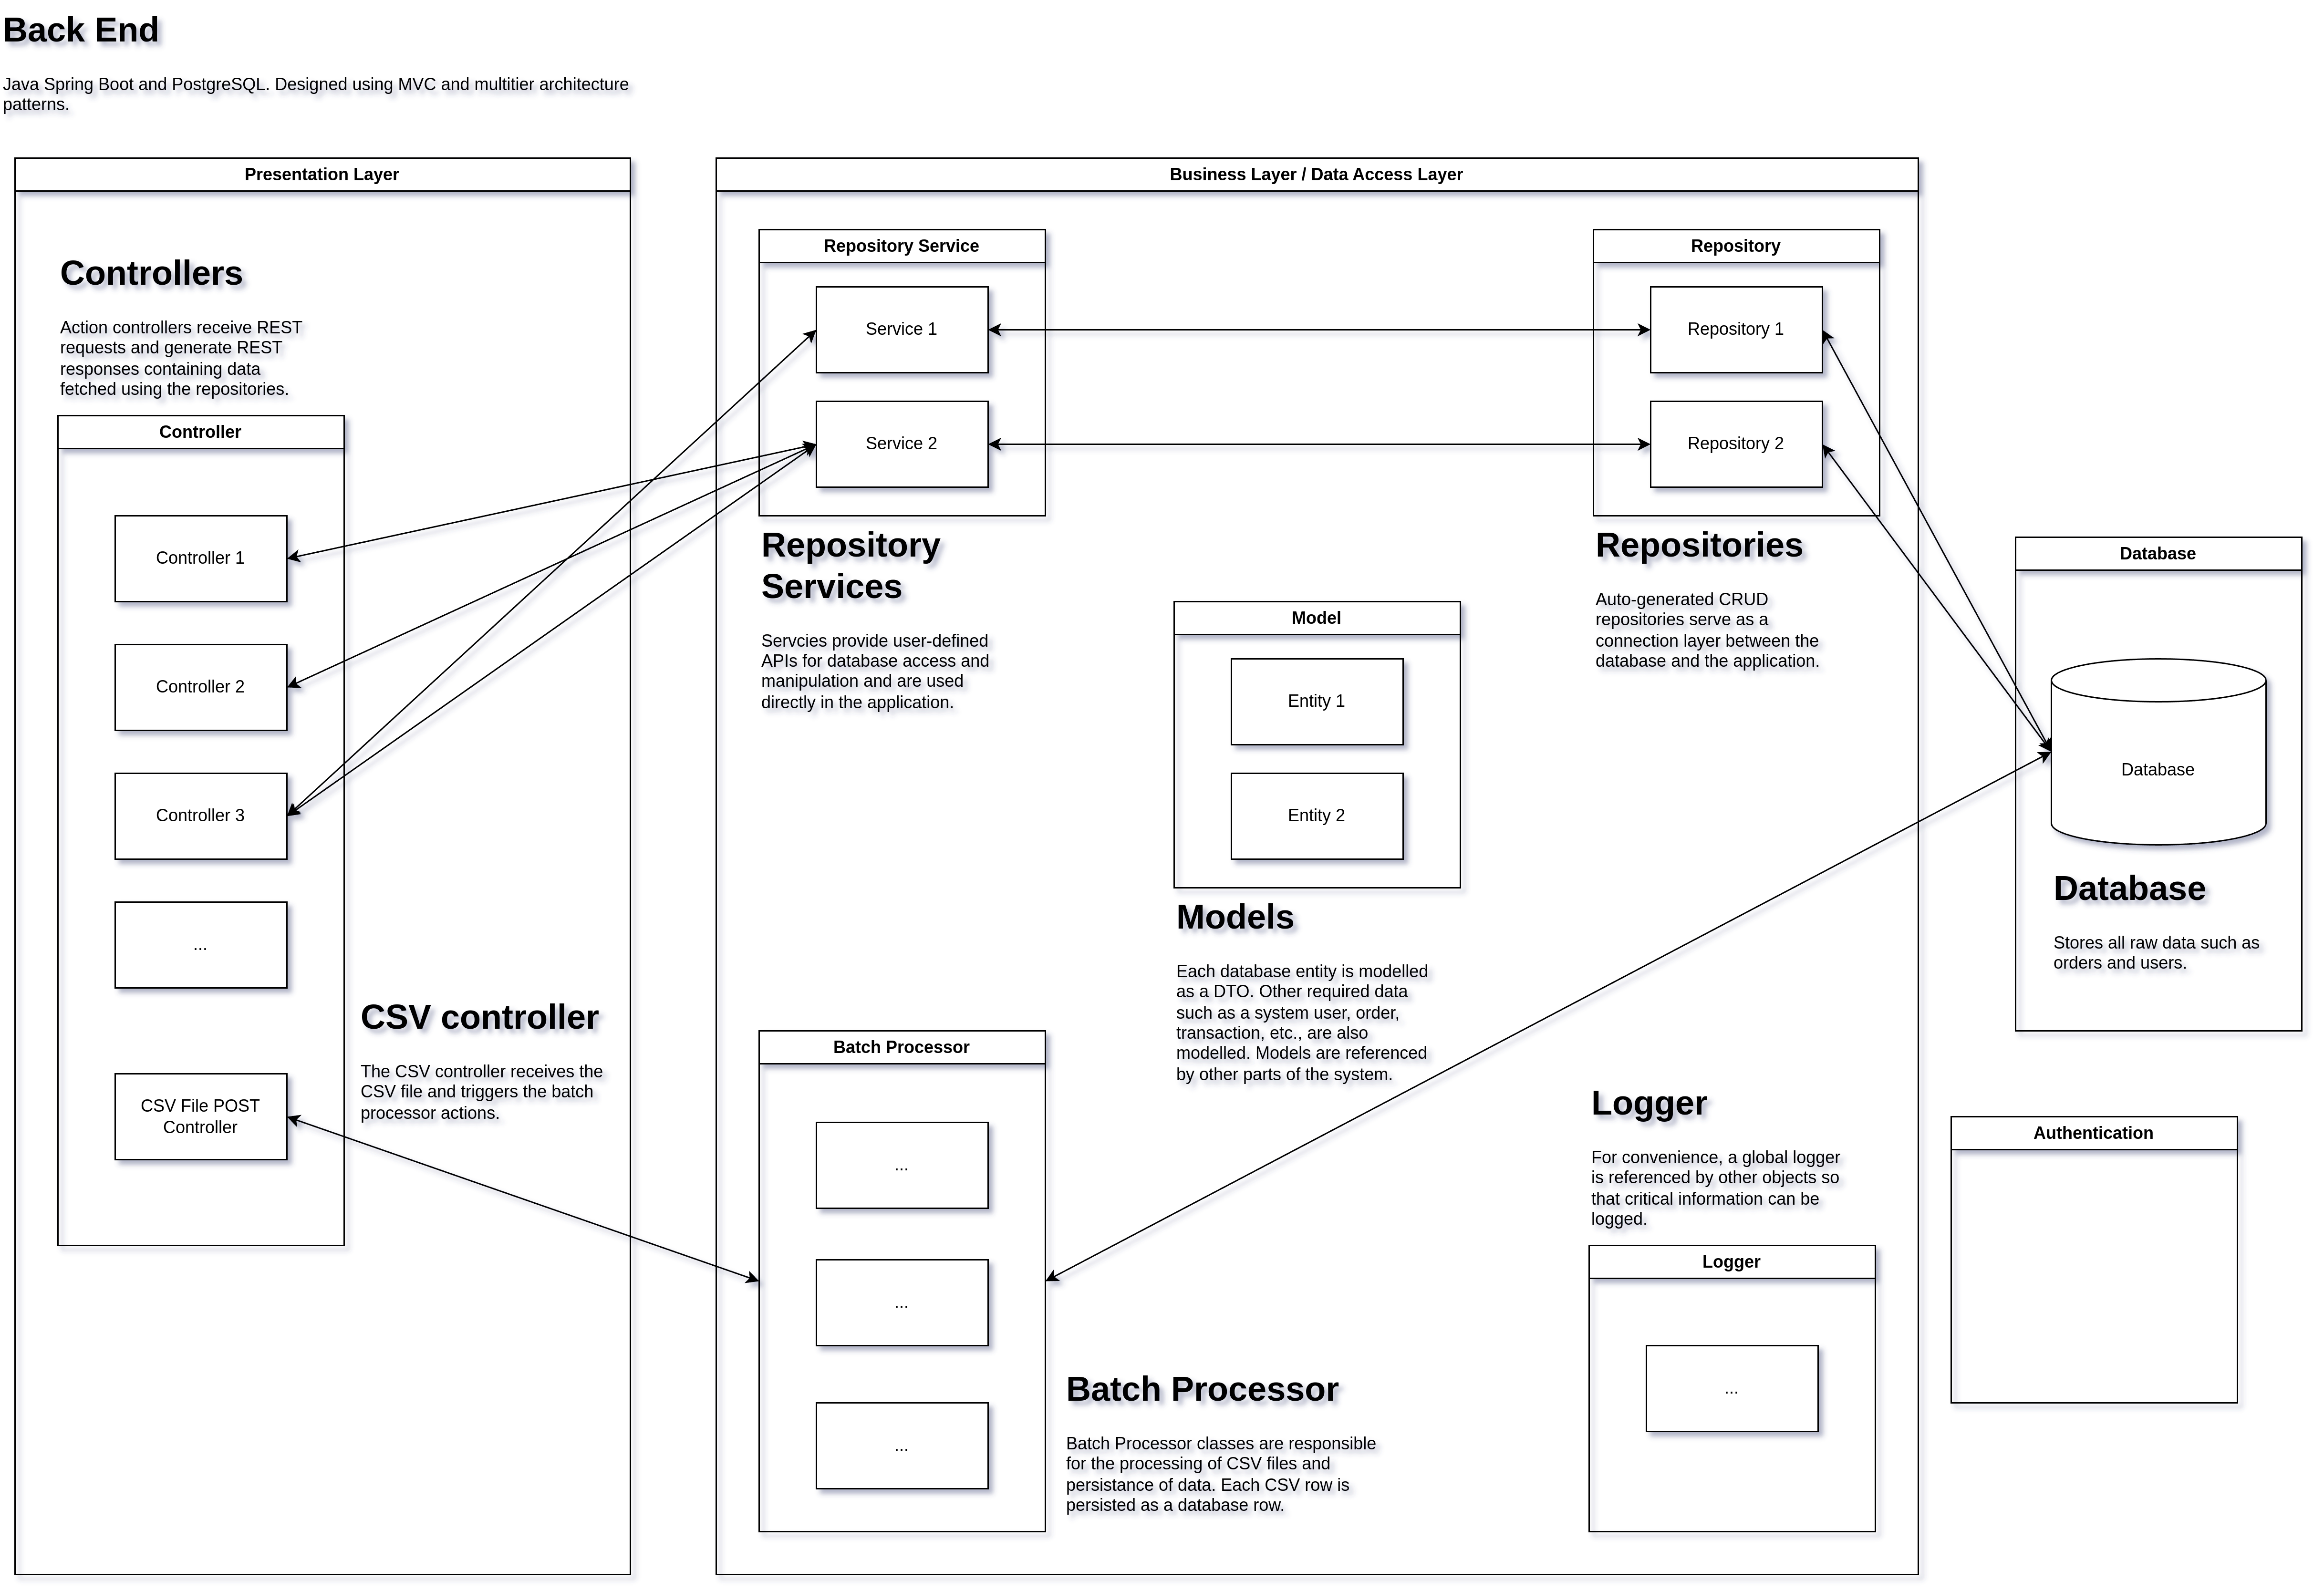
\includegraphics[width=\textwidth]{architecture-backend.png}
    \caption{The back end architecture.
    }\label{fig:architecture-backend}
\end{figure}
